\documentclass[10pt,twocolumn]{article}

\usepackage[margin=0.75in]{geometry}
\usepackage{times}
\usepackage{graphicx}
\usepackage{booktabs}
\usepackage{amsmath,amssymb}
\usepackage{enumitem}
\usepackage{xcolor}
\usepackage{url}
\usepackage[numbers,sort&compress]{natbib}
\usepackage[hidelinks]{hyperref}
\usepackage{microtype}
\usepackage{caption}
\captionsetup{font=small,labelfont=bf,skip=4pt}
\setlength{\columnsep}{0.25in}
\setlength{\parskip}{0pt}
\setlist[itemize]{leftmargin=*,itemsep=1pt,topsep=2pt,parsep=0pt}
\setlist[enumerate]{leftmargin=*,itemsep=1pt,topsep=2pt,parsep=0pt}
\newcommand{\ASS}{\mathrm{AS}_{\mathrm{SING}}}
\newcommand{\ASF}{\mathrm{AS}_{\mathrm{fair}}}
\newcommand{\HoldoutParagraph}{The E9 holdout (water, green, thin, knitted; 50 trials; linear and nonlinear plants) is running; results pending.}


\title{\vspace{-0.6em}Null-Space Energy Explains SING's Cross-Model Ranking:\\
An Audit of a Null-Space Leakage Score\vspace{-0.4em}}

\author{
Anonymous Authors\\
Workshop submission
}

\date{}

\begin{document}
\maketitle
\vspace{-1.2em}

\begin{abstract}
\vspace{-0.3em}
SING~\citep{sing2026} ranks 13 ImageNet classifiers by how much class-relevant semantics leak into the null space of their linear heads, and reports that a ``DinoViT'' leaks least.
Null-space energy accounts for this cross-model ranking.
The null energy fraction $\rho$ alone reproduces SING's published order as well as SING's own score does (Kendall $\tau{=}0.82$ for both).
Within a model, removing $d{=}1048$ rather than $d{=}24$ null dimensions raises $|$AS$|$ by ${\approx}10\times$ on 3 of 4 models; on BiT it drops instead, through translator conditioning.
Across controlled energy and dimension, $|$AS$|\propto\rho^{a}$ with $a\approx0.4$--$0.5$ (cell-bootstrap CI $[0.39,0.48]$), and high-variance null directions carry \emph{less} AS per unit $\sqrt{\rho}$ than random ones on 3 of 4 models, so energy acts as a confound rather than as signal.
Even the best planted-leakage score from our search (M1, post hoc) orders the 13 models much as $\rho$ does ($\tau{=}0.79$).
Second, SING's ``DinoViT'' cannot be identified as DINO: no public ViT-L/16 matches its reported 84.0\% top-1, and SING's translator fits the supervised timm AugReg checkpoint best (mean cosine $0.85$ vs.\ ${\le}0.68$).
Size-corrected scores give orders that differ from SING's, but none reverses it with confidence: the outcome depends on the normaliser, the energy-matched correction over-corrects, and model ranks shift with the null tolerance.
We report every pre-registered check, including the failures: a probe score (E8) and a 20-candidate score screen (E9) were KILLs, the flatness rule behind them is ill-posed, rank stability across null tolerances failed, and E3 and the flatness part of E1 did not pass.
We recommend reporting $\rho$ and an energy-only ranking alongside any cross-model null-space score.
\vspace{-0.3em}
\end{abstract}

\section{Introduction}
\vspace{-0.2em}
A linear classifier on features $f\in\mathbb{R}^m$ has a null space of dimension $m{-}\mathrm{rank}(W)$ that leaves the logits unchanged.
SING~\citep{sing2026} treats class-relevant content in that null space as ``leakage'': information the head could have used, but did not.
Its Absolute Shift (AS) measures how far a CLIP-aligned~\citep{clip2021} translation of $f$ moves once the null component is removed.
SING uses AS and the IS/AS ratio to rank 13 models, and singles out a ViT labelled ``DinoViT''~\citep{dino2021}.
Null spaces also show up in work on out-of-distribution failure~\citep{idnani2023}, outlier detection~\citep{vim2022,cook2020}, overfitting~\citep{rezaei2023} and information hiding~\citep{li2024null}.
In NLP, nullspace projection is used to remove a property from representations (INLP~\citep{ravfogel2020inlp}, amnesic probing~\citep{elazar2021amnesic}).
Work in that area has also established that probe readouts must be compared against controls~\citep{hewitt2019control}.
Representation-similarity scores are known to be dominated by high-variance directions~\citep{davari2023cka}.

Across architectures, the null dimension $d$ and the null energy fraction
$\rho = \mathbb{E}\|V_nV_n^\top f\|^2/\mathbb{E}\|f\|^2$
both vary by orders of magnitude.
If AS mostly tracks how much energy is removed, then a cross-model comparison of ``semantics'' is confounded by size.
We test this directly, and our experiments support it.

\paragraph{Contributions.}
(1)~\emph{Null energy explains SING's ranking} (\S\ref{sec:energy}): $\rho$ alone reproduces SING's 13-model order ($\tau{=}0.82$); AS grows with removed energy within a model (Exp~1) and scales as $\rho^{a}$, $a\approx0.4$--$0.5$, with resampled CIs (E1); top-variance null directions are not more semantic per unit energy; and the best planted-recovery score we found (M1) also tracks $\rho$.
(2)~\emph{The DinoViT identity} (\S\ref{sec:dino}): the checkpoint is not DINO, and SING's translator fits the timm AugReg ViT-L/16 best by a pre-registered margin.
(3)~\emph{Secondary, caveated}: size-corrected rankings differ from SING's under most normalisers, but no correction reverses it with confidence (\S\ref{sec:r2}). Under SING's own score, two class-level claims (C4, C8) do not reproduce on our pipeline.
(4)~We report every pre-registered experiment (Table~\ref{tab:prereg}), including two KILLs, a failed stability check and the flawed flatness rule behind the KILLs.

\begin{table*}[t]
\centering
\scriptsize
\setlength{\tabcolsep}{3pt}
\resizebox{\textwidth}{!}{%
\begin{tabular}{@{}llll@{}}
\toprule
Exp. & Pre-declared criterion (short) & Outcome & Where \\
\midrule
Exp~0 & null size correlates with SING IS/AS ($d_{\mathrm{null}}$; $\rho$ as baseline) & GO rests on $\rho$ ($-0.94$, E2 features); $d_{\mathrm{null}}$ alone $-0.46$, $p{=}0.12$ & \S\ref{sec:energy} \\
Exp~1 & $r{=}\mathrm{AS}(1048)/\mathrm{AS}(24)\ge3$ on $\ge3/4$ models and $\tau_{d=24}\le0.5$ & GO ($r\approx10$ on 3/4; BiT $0.06$; $\tau{=}0.29$) & \S\ref{sec:exp1} \\
E1 & ENERGY-DRIVEN: high/low $\ge3\times$ at fixed $d$ and $\le1.5\times$ across $d$ at fixed $\rho$ & MIXED (first part holds 4/4; second fails) & \S\ref{sec:e1} \\
E2 & $\tau(\ASF,\text{SING})\le0.5$ or $\ge1$ headline claim reverses & PASS as registered; weakened by round-2 tests (below) & \S\ref{sec:e2} \\
E3 & $\tau(\ASF,\text{planted})\ge0.8$ and $\tau(\ASS,\text{planted})\le0.5$ & Not passed ($0.109$ vs $0.386$); KILL condition ($\ASS\ge0.8$) not met & \S\ref{sec:e3} \\
E8 & NCP probe: $\tau\ge0.8$ and flat ($\max/\min\le1.5$ across $d$); KILL if $\tau<0.6$ & KILL ($\tau{=}{-}0.331$ $[-0.392,-0.273]$; flat 0/4) & \S\ref{sec:e8e9} \\
E9 & 20-candidate screen: DEV $\tau\ge0.8$ and flat on $\ge3/4$ at $\alpha\in\{0.1,1\}$ & KILL (best M1 $\tau{=}0.976$, flat 0/4). Post-hoc holdout: no candidate passes as registered; M1 $\tau{=}0.93$, passes only with revised flatness & \S\ref{sec:e8e9} \\
R2 & KILL-R: drop ``disagrees'' unless fix 2 and D-weak pass on all 13 and screened set & Not fired; ``differs from'' allowed & \S\ref{sec:r2} \\
R2 & D-strong (``reverses''): $\tau$ CI upper bound $<0$ under $\ge5/8$ normalisers & FAIL (0/8 all 13; 1/8 screened): no reversal claim & \S\ref{sec:r2} \\
R2 & $\ASF$ removes the $\rho$ trend: $|$Spearman$|<0.3$ and CI covers 0 & FAIL on screened set ($-0.79$ $[-1,-0.23]$): $\ASF$ over-corrects & \S\ref{sec:r2} \\
R2 & Tolerance stability: adjacent-tolerance $\tau\ge0.9$ for every score & FAIL ($\ASF$ $0.87$/$0.82$; $\ASS$ $0.87$ on all 13); $\rho$ $0.92$/$1.00$ & \S\ref{sec:r2} \\
R2 & PC bands: $G_{\mathrm{top}}/G_{\mathrm{rand}}$ CI vs 1 on $\ge3/4$ models at $d{=}24$ & Top PCs carry less AS per unit energy (3/4; ResNet50 the exception) & \S\ref{sec:e1} \\
R2 & Synthetic oracle passes the E8/E9 flatness rule & FAIL (ratio $3.55$ / $3.48$): rule ill-posed & \S\ref{sec:e8e9} \\
R2 & DinoViT translator fidelity: used checkpoint best by $\ge0.05$ & PASS ($0.848$ vs.\ next best $0.677$; margin $0.171$) & \S\ref{sec:dino} \\
\bottomrule
\end{tabular}}
\vspace{-0.4em}
\caption{All pre-registered experiments and their outcomes. Pre-registrations and results are in the repository (\texttt{FULL\_PAPER\_PLAN.md}, \texttt{e8/PREREG\_E8.md}, \texttt{E9\_SCORE\_SCREEN\_PREREG.md}, \texttt{PREREG\_R2.md}). R2 = the round-2 pre-registration written in response to review.}
\label{tab:prereg}
\vspace{-0.8em}
\end{table*}

\section{Background}
\label{sec:bg}
\vspace{-0.2em}
\paragraph{SING AS in brief.}
Let $T(f)=Af+b$ be SING's released linear translator into CLIP space and $V_n$ an orthonormal basis of $\ker(W)$ (singular-value tolerance $10^{-5}$ unless stated).
For a text direction $t$, the per-image absolute shift is the change in angle $\theta(T(f),t)$ after removing $V_nV_n^\top f$.
$\ASS$ denotes the image-averaged $|$AS$|$ under full null removal, with class text as the target.
We match SING's released code (commit \texttt{e47b37d}) on a fixed 10k ImageNet-val subset (10 images/class), plus a 200-image claim-class set (all 50 val images each of jellyfish, porcupine, Arabian camel and sports car), and recompute every score for all 13 released translators.
SING itself is not consistent about its protocol. Its text mentions a ``12-model sweep'' while Supp.\ Table~3 lists 13 models. It describes 16 classes in one place and 10k features over 1000 classes in another. Its bibliography gives the wrong arXiv id for \citep{li2024null}.

\section{Null energy explains SING's ranking}
\label{sec:energy}
\vspace{-0.2em}
\paragraph{$\rho$ alone reproduces the order.}
We digitised the 13 IS/AS bars in SING Supp.\ Fig.~12b (the extended ratio comparison).
Against this order, $\tau(\ASS){=}0.821$ (model-bootstrap 95\% CI $[0.56,1]$), which reproduces SING.
Ranking models by $\rho$ alone gives the same $\tau{=}0.821$ $[0.56,1]$ (Fig.~\ref{fig:norm}); on the screened set of \S\ref{sec:r2} it gives $0.78$ $[0.44,1]$, against $0.82$ $[0.51,1]$ for $\ASS$.
Over 13 models, Spearman$(\rho,\ASS){=}0.87$ and Spearman$(\rho,\mathrm{IS}/\mathrm{AS}){=}{-}0.94$ ($p{=}1.9{\times}10^{-6}$).
Null dimension alone does not explain the order (Spearman $-0.46$, $p{=}0.12$; DenseNet null dim $27$ at tol $10^{-5}$): DeiT3-L~\citep{deit3} has null dim $24$ yet the worst ratio.
SING's model order therefore matches the order that null energy alone predicts.
Unlike either score, the $\rho$ ranking is also stable across null tolerances (adjacent-tolerance $\tau\ge0.92$; \S\ref{sec:r2}).

\subsection{Within-model size dependence (Exp~1)}
\label{sec:exp1}
On the 10k subset we remove random $d$-dimensional subspaces of each model's own null space ($d\in\{24,48,100,280,536,1048\}$, 20 seeds for $d{<}d_{\mathrm{null}}$). The models are ResNet50, ResNeXt101, BiT-R50x1~\citep{bit2020} and DINOv2-L~\citep{dinov2}, all with $d_{\mathrm{null}}{=}1048$, and SING's released translators.
The ratio is $r\approx10$ on 3 of 4 models (Fig.~\ref{fig:exp1}).
Because random sub-subspaces remove energy nearly linearly in $d$, the fits against $d$ and against $\rho_d$ are indistinguishable ($R^2$ in Table~\ref{tab:exp1}), and Exp~1 by itself cannot separate them.
At matched $d{=}24$ across 8 models, Kendall $\tau$ against the Supp.\ Fig.~12b order is $0.29$ ($p{=}0.40$).

\begin{figure}[t]
\centering
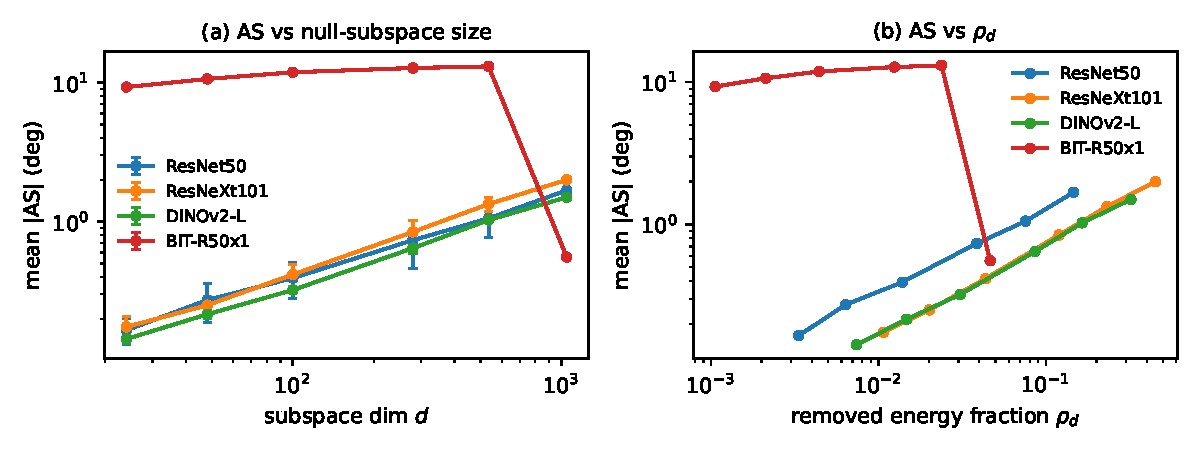
\includegraphics[width=\linewidth]{figs/fig_exp1_curves.pdf}
\vspace{-0.4em}
\caption{Exp~1: mean $|$AS$|$ vs.\ subspace size $d$ (a) and removed energy $\rho_d$ (b). BiT collapses at the full null (translator cancellation).}
\label{fig:exp1}
\vspace{-0.6em}
\end{figure}

\begin{table}[t]
\centering
\scriptsize
\setlength{\tabcolsep}{3pt}
\begin{tabular}{@{}lccc@{}}
\toprule
Model & $r$ & $2\sigma$ band & $R^2$ (vs $d$ $\equiv$ vs $\rho_d$) \\
\midrule
ResNet50   & 10.15 & $[5.83,14.48]$ & 0.983 \\
ResNeXt101 & 11.44 & $[6.93,15.95]$ & 0.977 \\
DINOv2-L   & 10.48 & $[8.85,12.10]$ & 0.974 \\
BiT-R50x1  & 0.060 & $[0.057,0.063]$ & 0.512 \\
\bottomrule
\end{tabular}
\vspace{-0.4em}
\caption{Exp~1: $r{=}\mathrm{AS}(1048)/\mathrm{AS}(24)$. For random sub-subspaces $\rho_d$ is linear in $d$, so the two $R^2$ coincide.}
\label{tab:exp1}
\vspace{-0.8em}
\end{table}

\paragraph{BiT anomaly.}
BiT's full-null AS collapses ($r{=}0.06$), even though partial subspaces give large AS ($9$--$13^\circ$).
The singular values of $AV_n$ are extreme (top $284$ vs.\ $5.6$ for ResNet50), and the orthogonal null blocks nearly cancel through the translator.
BiT also fails our degeneracy screen: a retained row-space direction with $\sigma{=}8.9{\times}10^{-4}$ carries 26\% of the feature energy.

\subsection{Energy vs.\ dimension (E1)}
\label{sec:e1}
\paragraph{Geometry.}
If a linear translator maps a removed component of relative energy $\rho$ into CLIP space and the residual is small relative to $\|T(f)\|$, the first-order angular change scales with $\|\Pi f\|\propto\sqrt{\rho}$, i.e.\ exponent $0.5$.
\paragraph{Design and result.}
On ResNet50, ResNeXt101, DINOv2-L, VGG16 and EVA02-L we compare high- with low-energy null PCs at fixed $d\in\{24,100,280\}$, and hit fixed $\rho\in\{0.5\%,2\%,8\%\}$ at several $d$ by mixing top and bottom PCs.
The pooled fit over 76 cells, $\log|\mathrm{AS}|=a\log\rho+b\log d+c_{\mathrm{model}}$, gives $a{=}0.431$ and $b{=}0.010$ ($R^2{=}0.93$; Fig.~\ref{fig:e1}).
The cell-level bootstrap gives $a\in[0.388,0.485]$ and the model-clustered bootstrap gives $[0.382,0.464]$. Leaving one model out gives $a\in[0.408,0.452]$, and per-model fits give $0.38$--$0.46$. $b$ covers $0$ under both bootstraps.
We therefore claim only $a\approx0.4$--$0.5$.
At fixed $d$, the high/low ratio exceeds $3\times$ on all 4 evaluable models. At fixed $\rho$, however, the max/min across $d$ exceeds $1.5$ in several cells (up to $2.29$). We therefore rate E1 as \textbf{mixed}: energy dominates the fit, and the pre-registered flatness part still fails.

\begin{figure}[t]
\centering
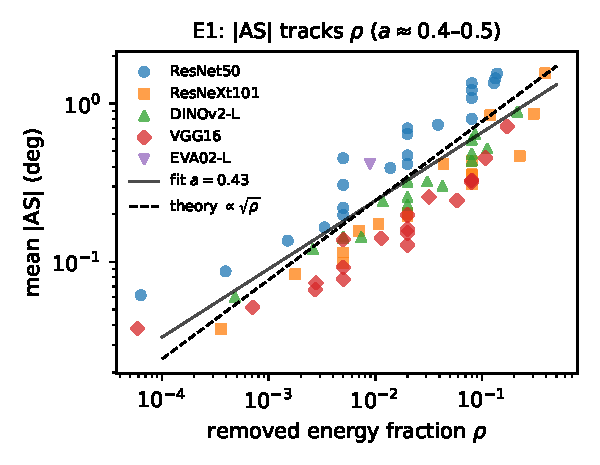
\includegraphics[width=0.85\linewidth]{figs/fig_e1_energy.pdf}
\vspace{-0.4em}
\caption{E1 cells: $|$AS$|$ vs.\ $\rho$. Solid: pooled fit ($a{=}0.43$, cell bootstrap $[0.39,0.48]$); dashed: $\sqrt{\rho}$.}
\label{fig:e1}
\vspace{-0.6em}
\end{figure}

\paragraph{Energy as confound or as signal (round 2).}
If high-variance null directions were the semantic ones, energy would partly \emph{be} the signal.
At matched $d$, we compare $G{=}\mathrm{AS}/\sqrt{\rho}$ for the top-variance null PCs against random null sub-subspaces (1000$\times$ image bootstrap).
At $d{=}24$, $G_{\mathrm{top}}/G_{\mathrm{rand}}$ is $0.60$ (ResNeXt), $0.87$ (DINOv2) and $0.008$ (BiT), all with CIs below 1, but $1.16$ $[1.15,1.17]$ for ResNet50. At $d{=}100$: $1.01$, $0.85$, $0.83$, $0.011$.
Top PCs therefore carry \emph{less} AS per unit $\sqrt{\rho}$ than random directions on 3 of 4 models. High-energy directions are not disproportionately semantic, which supports the confound reading.
$G$ is not constant across bands, though, so $\sqrt{\rho}$ is only an approximate nuisance model.

\paragraph{The best planted-recovery score also tracks $\rho$.}
M1, the only score from our search that recovers planted leakage well (\S\ref{sec:e8e9}), orders the 13 models close to $\rho$ ($\tau{=}0.79$, Spearman $0.90$; screened $0.75$, $0.85$), and its $\tau$ against SING, $0.667$ $[0.29,0.94]$, has a CI that includes $\ASS$'s $0.821$.
M1 is post hoc and is used here only descriptively (\S\ref{sec:e8e9}).

\section{The DinoViT identity}
\label{sec:dino}
\vspace{-0.2em}
SING reports DinoViT at 84.0\% top-1 (Supp.\ Table~3).
The released \texttt{models.yaml} loads a timm AugReg ViT-L/16, while the wrapper in the supplement uses torchvision attribute names.
We evaluated five public ViT-L/16 candidates on the full 50k validation set:
torchvision IMAGENET1K\_V1 (79.67\%),
timm AugReg (85.85\%),
SWAG linear~\citep{swag2022} (85.14\%),
SWAG E2E (88.07\%)
and HF \texttt{google/vit-large-patch16-224} (81.98\%).
None falls in $84.0\pm0.3$ (Fig.~\ref{fig:exp0b}). All five are supervised or SWAG weakly supervised, and DINO never released a ViT-L with a 1000-way head~\citep{dino2021}.
The checkpoint we use (timm AugReg, the one SING's \texttt{models.yaml} loads) gives mean $\cos(T(f),\mathrm{CLIP})=0.848$ with SING's \texttt{dinovit1} translator.
On the first 1000 subset images, re-extracted with each candidate's native transform, the other four give $0.677$ (torchvision IMAGENET1K\_V1), $0.631$ (HF), $0.615$ (SWAG linear) and $0.608$ (SWAG E2E). The used checkpoint is best by $0.171$, above the pre-registered $0.05$ margin. Its re-extracted features match our cached ones exactly. These results suggest that SING's translator was fit on this timm AugReg model, irrespective of its DinoViT label.

\begin{figure}[t]
\centering
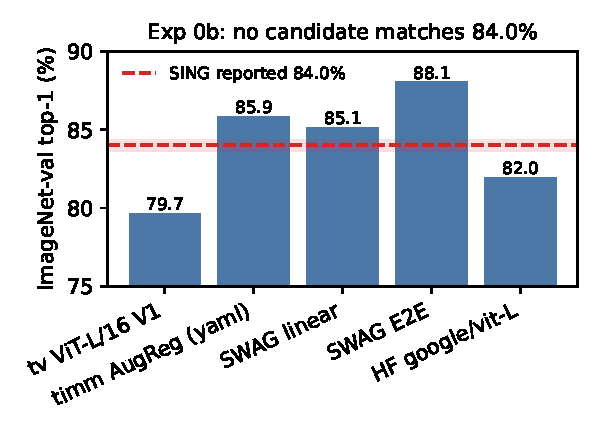
\includegraphics[width=0.85\linewidth]{figs/fig_exp0b.pdf}
\vspace{-0.4em}
\caption{Exp~0b top-1 on ImageNet-val (native eval transform). No candidate matches SING's reported 84.0\%.}
\label{fig:exp0b}
\vspace{-0.6em}
\end{figure}

\section{Secondary: size-corrected rankings (E2, round 2)}
\label{sec:e2}\label{sec:r2}\label{sec:fair}
\vspace{-0.2em}
We now examine whether removing the energy dependence leaves a confident alternative ranking. None of the corrections we tried does.

\paragraph{Size-fair scores.}
$\ASF = \mathrm{AS}_{\mathrm{null}}/\mathrm{AS}_{\mathrm{rand}}$, where $\mathrm{AS}_{\mathrm{rand}}$ is the mean $|$AS$|$ after removing an energy-matched random subspace.
In the original analysis (\emph{family A}), the random subspace is Haar over the full feature space (seed $10000{+}r$, 20 draws).
Because this changes the logits, in round 2 we added two control families that preserve them better.
\emph{Family B} draws an energy-matched subspace from the span of the lowest-$\sigma$ row-space directions of $W$. These directions do change the logits, by up to $14$--$74$ logit SDs for models with a large span (VGG, ResNeXt).
\emph{Family C} compares a random $24$-dim null sub-subspace, which changes no logit, against a family-B control of matched energy.
Every score is reported on all 13 models and on a pre-declared \emph{screened} set of 11. The screen excludes models with $\rho{<}10^{-4}$ or with a retained direction of $\sigma{<}10^{-3}$ holding ${>}5\%$ of the energy, which removes DenseNet ($\rho{=}1.8{\times}10^{-8}$) and BiT.

\begin{figure*}[t]
\centering
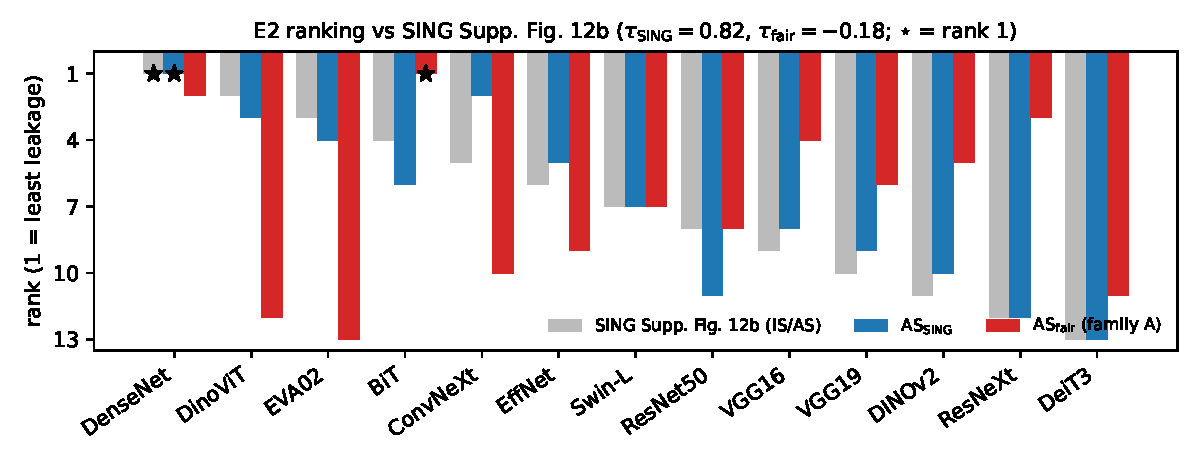
\includegraphics[width=0.49\linewidth]{figs/fig_e2_ranking.pdf}\hfill
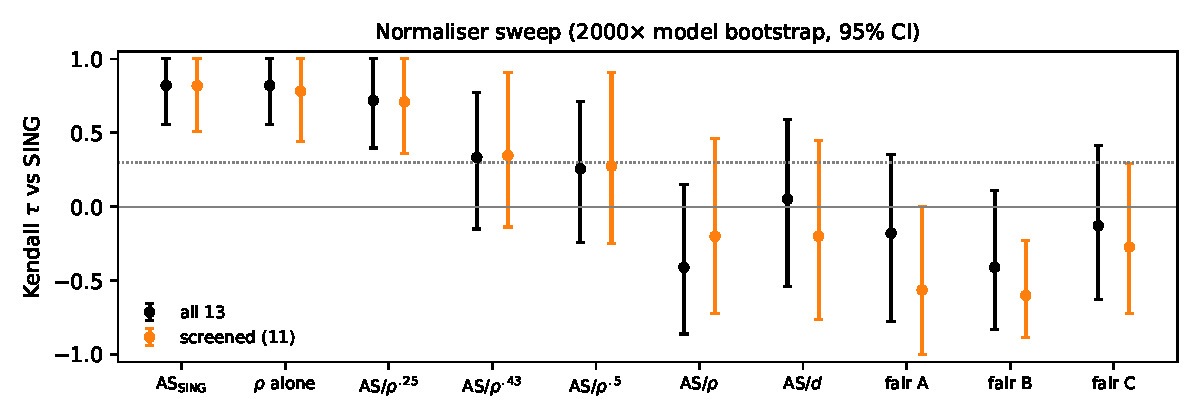
\includegraphics[width=0.49\linewidth]{figs/fig_r2_normalisers.pdf}
\vspace{-0.4em}
\caption{Left: ranks (1 $=$ least leakage, $\star$ marks rank 1) under SING Supp.\ Fig.~12b, $\ASS$ and $\ASF$ (family A). Right: $\tau$ vs.\ SING for each normaliser and for $\rho$ alone, with 2000$\times$ model-bootstrap 95\% CIs, on all 13 models and on the screened 11. Dotted line: the $\tau{=}0.3$ bar of fix 2.}
\label{fig:e2rank}\label{fig:norm}
\vspace{-0.6em}
\end{figure*}

\paragraph{Do size corrections change the order?}
Point $\tau$ vs.\ SING is $-0.18$ (family A), $-0.41$ (B) and $-0.13$ (C) on all 13 models, and $-0.56$, $-0.60$ and $-0.27$ on the screened set. All are below the pre-registered $0.3$ bar.
Over eight normalisers (AS$/\rho^{a}$ for $a\in\{.25,.43,.5,1\}$, AS$/d$, families A--C), the 95\% CI excludes $\ASS$'s $0.821$ for 7 of 8 normalisers on all 13 models (D-weak passes). On the screened set it does so for exactly 5 of 8, which is the minimum the rule allows.
The stronger, pre-registered reversal criterion (D-strong: CI entirely below $0$ under ${\ge}5/8$) fails: no normaliser meets it on all 13, and only family B does on the screened set ($[-0.89,-0.23]$).
Normalising by the fitted exponent leaves a positive $\tau$ ($\rho^{0.43}$: $+0.33$ $[-0.15,0.77]$; $\sqrt{\rho}$: $+0.26$), so the answer depends on which normaliser is chosen.
The data support only the claim that size-corrected rankings \emph{differ from} SING's; we make no reversal claim.

\paragraph{$\ASF$ over-corrects.}
Spearman$(\ASF,\rho)$ is $-0.26$ $[-0.96,0.41]$ on all 13 models and $-0.79$ $[-1,-0.23]$ on the screened set (Fig.~\ref{fig:e2sc}b).
Low-$\rho$ models such as DinoViT and EVA02 are pushed to the bottom. Instead of removing the energy trend, $\ASF$ inverts it.

\paragraph{Tolerance sensitivity (pre-registered check failed).}
At null tolerances $10^{-6}$ to $10^{-3}$, the null dimension of DenseNet grows from 25 to 221, while that of the other models barely changes.
Rank agreement between adjacent tolerances drops below the pre-registered $0.9$ for both scores: $\ASF$ gives $0.87$ (all 13) and $0.82$ (screened) from $10^{-5}$ to $10^{-4}$, and $\ASS$ gives $0.87$ from $10^{-4}$ to $10^{-3}$. Null dim and $\rho$ stay at or above $0.92$. The check fails. Model rankings from either score are therefore not reliable to single-rank precision.

\begin{figure}[t]
\centering
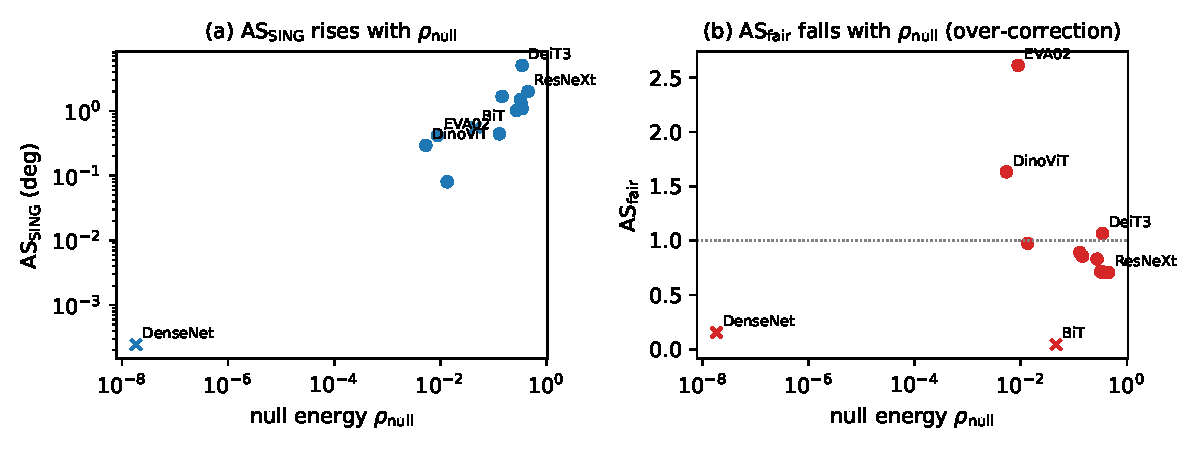
\includegraphics[width=\linewidth]{figs/fig_e2_scatter.pdf}
\vspace{-0.4em}
\caption{(a)~$\ASS$ rises with $\rho_{\mathrm{null}}$. (b)~$\ASF$ (family A) falls with $\rho_{\mathrm{null}}$: it over-corrects (Spearman $-0.79$ on the screened set). $\times$: models excluded by the degeneracy screen.}
\label{fig:e2sc}
\vspace{-0.6em}
\end{figure}

\paragraph{Class-level claims.}
For each claim we define a signed effect (positive $=$ SING's direction) and bootstrap images within class (1000$\times$, seed 0). A claim \emph{holds} if the CI is above $0$, \emph{reverses} if it is below, and is \emph{not confirmed} if the CI covers $0$ (Table~\ref{tab:claims}).
These CIs capture image resampling only, not the choice of model set or normaliser, so they are narrow.
Under $\ASS$, two claims do not reproduce on our pipeline:
\begin{itemize}
\item \textbf{C4}: DinoViT does not have the lowest class AS (effect $-0.29^\circ$); ConvNeXt and DenseNet are lower.
\item \textbf{C8}: ResNet's porcupine and sports-car classes are not in the top decile (percentile gaps $-5.2$ $[-9.7,-2.4]$ and $-29$).
\end{itemize}
C10 (jellyfish $\gg$ camel) is not confirmed ($-0.11$ $[-0.21,0.001]$).
These discrepancies between SING and our re-implementation may reflect protocol differences (SING used ${\approx}30$ concepts and ${\approx}1300$ images for C10). They do not arise from size correction.
Under $\ASF$, the image-bootstrap CIs of the other testable claims lie on the opposite side, C12 is not confirmed under the model bootstrap, and C9 (``no correlation'') is contradicted. Because $\ASF$ over-corrects, we treat these as diagnostics and do not claim class-level reversals.
By $\ASF$ (family A), DinoViT ranks 12th of 13; under $\ASS$ it ranks 3rd.

\paragraph{DinoViT ratio gap.}
Our DinoViT IS/$|$AS$|$ is $20.95$, against $70.16$ in Supp.\ Fig.~12b, a $3.35\times$ gap. For the other 12 models SING's ratio is $0.98$--$2.5\times$ ours (EVA02 $2.5\times$, BiT $1.9\times$, DenseNet $1.7\times$), so the gap is largest for DinoViT, while the $\ASS$ order still agrees.
The gap could reflect differences in SING's image and class subset (16 classes vs.\ our 1000), its concept set, or its checkpoint (\S\ref{sec:dino}). We cannot tell them apart without SING's evaluation lists.

\begin{table}[t]
\centering
\scriptsize
\setlength{\tabcolsep}{2pt}
\resizebox{\linewidth}{!}{%
\begin{tabular}{@{}cllcc@{}}
\toprule
ID & Claim (short) & Effect $\ASS$ [95\% CI] & $\ASS$ & $\ASF$ \\
\midrule
C1 & DinoViT best ratio (proxy) & $+0.149$ $[.142,.156]$ & holds & opp. \\
C2 & ResNeXt worst ratio (proxy) & $+0.323$ $[.302,.342]$ & holds & opp. \\
C3 & ResNet $>$ DinoViT & $+1.383$ $[1.37,1.39]$ & holds & opp. \\
C4 & DinoViT least leakage & $-0.293$ $[-.298,-.289]$ & \textbf{rev.} & opp. \\
C5 & ResNeXt top-2 of 5 & $+1.442$ $[1.42,1.46]$ & holds & opp. \\
C6 & ResNet per-class $>$ DinoViT & mean $+1.38$, SD $+0.74$ & holds & opp. \\
C7 & DinoViT per-class $|$AS$|{<}1^\circ$ & $+0.50$ $[.497,.50]$ & holds & n/a \\
C8 & Porcupine/sports car $\ge$90th pct & $-5.2$ / $-29$ pct & \textbf{rev.} & opp. \\
C9 & No ResNet--DinoViT class corr. & $-0.033$ $[-.056,.009]$ & holds & contra. \\
C10 & Jellyfish $\gg$ camel & $-0.107$ $[-.206,.001]$ & n.c. & opp. \\
C11 & DinoViT least steerable (proxy) & $+0.149$ $[.142,.156]$ & holds & opp. \\
C12 & Supp.\ Fig.~12b order ($\tau$) & $0.821$ $[.56,1]^{\dagger}$ & holds & n.c.$^{\dagger}$ \\
C13 & EVA02 target-space order & -- & untestable & untestable \\
\bottomrule
\end{tabular}}
\vspace{-0.4em}
\caption{E2 claim audit (round 2). rev.\ $=$ CI on the opposite side of $0$; n.c.\ $=$ not confirmed; opp.\ $=$ opposite side under $\ASF$, which over-corrects (Fig.~\ref{fig:e2sc}b), so these are diagnostics, not reversals; contra.\ $=$ a correlation is found. C7 has no $\ASF$ analogue ($\ASF$ is unitless). $^{\dagger}$Model bootstrap; $\ASF$ $\tau{=}{-}0.18$ $[-0.78,0.35]$. C1/C2/C11 use $|$AS$|$ proxies.}
\label{tab:claims}
\vspace{-0.8em}
\end{table}

\section{Planted leakage (E3)}
\label{sec:e3}
\vspace{-0.2em}
We plant a CLIP concept direction (\texttt{red}/\texttt{striped}/\texttt{water}) into the null spaces of 8 models, at log-uniform $\alpha\in[0.01,1]$ over 50 trials (plant seed $0$, bootstrap seed $1$). The logits stay unchanged (max $|\Delta\mathrm{logit}|\le2.3{\times}10^{-5}$).
Both scores are $\alpha{=}0$-subtracted per (model, concept).
Kendall $\tau$ against the planted ranking, averaged over concepts, is $0.386$ $[0.324,0.448]$ for $\ASS$ and $0.109$ $[0.046,0.171]$ for $\ASF$. Without the subtraction, $\ASF$ gives $0.071$ $[0.004,0.141]$.
Without DenseNet, the values are $0.343$ and $0.135$.
Neither score recovers planted strength well, so a size correction should not be read as a leakage oracle.

\section{Score search: E8, E9 and the flatness rule}
\label{sec:e8e9}
\vspace{-0.2em}
\paragraph{E8 (pre-registered, KILL).}
A probe-based null-content score (NCP: ridge-probe $R^2$ on null coordinates, $z$-scored against energy-matched random subspaces) gave $\tau{=}{-}0.331$ $[-0.392,-0.273]$ on the E3 planted task, and was flat on 0/4 eligible models.
Three implementation flags apply. The $z$-score saturates because both $R^2$ values approach 1. $\lambda$ was chosen by approximate closed-form LOO rather than the exact CV in the pre-registration. And $\lambda$ sat at the grid floor in 18 of 96 fits.
\paragraph{E9 (pre-registered, KILL).}
We screened 20 candidate scores on two DEV concepts. The rule was DEV $\tau\ge0.8$ and flatness ($\max/\min\le1.5$ across nested null sub-subspaces) on $\ge3/4$ models at both $\alpha\in\{0.1,1\}$.
No candidate qualified.
The best was M1 (debiased null leakage, $\hat L^2=(\|\sum_iPf_is_i\|^2-\sum_i\|Pf_i\|^2s_i^2)/(n(n{-}1)\mathbb{E}\|f\|^2)$ with standardised concept scores $s_i$; score $\sqrt{\max(\hat L^2,0)}$), with DEV $\tau{=}0.976$ $[0.963,0.988]$ but flat on 0/4.
Others: M2 $0.540$, S9 (a mutual-information score) $0.522$, S10 $0.395$ (the only flat one), M5 ($\mathrm{AS}/\sqrt{\rho}$) $0.323$, S4 ($\mathrm{AS}/\rho$) $-0.051$.
\paragraph{The flatness rule is ill-posed (round 2).}
On synthetic Gaussian features with a known head ($m{=}400$, null dim $300$), we planted a direction either in the full null or in a fixed 24-dim sub-subspace. We then scored an exact oracle, the planted amplitude inside the removed subspace $B$, $\alpha\|B^\top u\|$.
The oracle itself fails the rule, with $\max/\min$ $3.55$ and $3.48$ ($\approx\sqrt{300/24}$), because a larger $B$ contains more of the plant.
A revised rule, $\max/\min$ of score$/$oracle $\le1.5$, is passed by M1 in both settings (ratios $1.00$--$1.03$).
Re-judged post hoc on the saved DEV values, M1 is revised-flat on 4/4 models at both $\alpha$ and is the only E9 candidate that qualifies. E8's NCP is flat on 0/4. This is exploratory, and E8 and E9 remain KILLs as registered.
\paragraph{E9 holdout (round 2, post hoc).}
\HoldoutParagraph
\HoldoutTable
\paragraph{M1 on the 13 models (descriptive).}
We also rank the 13 models by M1 (post hoc, descriptive; \texttt{r2/e2\_m1.py}), since M1 beats $\ASF$ on the holdout.
At $\alpha{=}0$, on the full null and averaged over SING's 173 concepts, M1 gives $\tau{=}0.667$ $[0.29,0.94]$ against SING's order ($0.600$ $[0.06,0.92]$ on the screened set). Both intervals include $\ASS$'s $0.821$.
M1's order is close to $\rho$'s ($\tau{=}0.79$, Spearman $0.90$; screened $0.75$, $0.85$). We expected this, because M1 is scaled by total feature energy and not by null size. It gives no ranking that differs from SING's, and we treat it as a candidate for a future pre-registered test rather than as a recommended score: it was chosen post hoc, fails the registered flatness rule, and sees the concept score that defines the plant.

\section{Discussion}
\vspace{-0.2em}
SING's cross-model ranking is what null energy alone predicts: $\rho$ reproduces its order to the same $\tau$, AS grows with removed energy within a model, and the pooled energy exponent is close to the first-order $\sqrt{\rho}$ prediction with no detectable dimension effect.
Top-variance null directions are not more semantic per unit energy than random ones, which argues against reading energy as signal, and the one score that recovers planted leakage well (M1) also orders models by $\rho$.
This does not show that SING's ranking is wrong. It shows that the ranking cannot be told apart from an energy ranking.
Removing energy does not yield a confident alternative either. Energy-matched corrections either over-correct ($\ASF$) or leave a positive $\tau$ ($\rho^{0.43}$), and score-based model ranks shift with the null tolerance.
Within a model, AS remains a useful probe of null content as seen through the translator.

\paragraph{Recommendations.}
\begin{enumerate}
\item Name the exact checkpoint and its measured top-1.
\item Report $d_{\mathrm{null}}$, $\rho_{\mathrm{null}}$ and the null tolerance next to any null-space score, and check rank stability across tolerances.
\item Compare any cross-model score against the ranking by $\rho$ alone, as a control in the sense of~\citep{hewitt2019control}.
\item Flag translator conditioning when full-null and block-wise AS disagree (BiT).
\item Prefer within-model interventions to cross-architecture league tables.
\item Validate flatness or invariance criteria on a synthetic oracle before using them to accept or reject scores.
\end{enumerate}

\paragraph{Limitations.}
E1 does not cleanly separate energy from dimension, and its pre-registered flatness part fails.
The claim CIs reflect image resampling only.
Several claims rely on proxies (C1/C2/C11), and C13 is untestable.
The E9 holdout and the revised flatness rule are post hoc.
In the holdout, M1 is given the concept score that defines the plant, and the AS-family scores are not. The translator-fidelity check uses 1000 images.
We did not retrain translators or evaluate a true DINO model~\citep{dino2021}.
Nor did we extend the audit to other null-space scores~\citep{vim2022,cook2020,rezaei2023}, or to information-theoretic leakage measures for concept models~\citep{makonnen2025}, which target a different notion of leakage.

\section{Conclusion}
\vspace{-0.2em}
Using the released translators, we reproduce SING's 13-model ranking and find that null-space energy $\rho$ alone reproduces it equally well; within-model, energy-controlled and PC-band tests all point to energy as a confound.
SING's ``DinoViT'' is a supervised timm AugReg ViT-L/16, not a DINO model.
Size-corrected scores produce orders that differ from SING's, but none reverses it with confidence.
We report all pre-registered experiments, including the two KILLs (E8, E9), the failed tolerance-stability check and the flaw in the shared flatness criterion.
Cross-model null-space comparisons should report $\rho$ and an energy-only baseline next to the score.

\vspace{0.4em}
\noindent\textbf{Reproducibility.}
Code, aggregated results, pinned environment, the image-subset list and a one-command \texttt{make reproduce} are at \url{https://github.com/sudeshgm/ic014-sing-null-dimension}.
ImageNet-derived features are not redistributed; checksums and the extraction scripts are provided.

{\small
\bibliographystyle{plainnat}
\bibliography{refs}
}

\appendix
\section{Additional numerical detail}
\vspace{-0.2em}
\paragraph{Seeds.}
AS$_{\mathrm{rand}}$ family A: $10000{+}r$, $r{<}20$. Family B: $50000{+}r$. Family C sub-subspaces: $30000{+}j$, controls $60000{+}j$. Exp~1 subspaces: 20 seeds per $d$. E3 plants: seed 0 (log-uniform $\alpha$), bootstrap 10000$\times$ seed 1. Model bootstrap: 2000$\times$ seed 0. Claim bootstrap: 1000$\times$ seed 0. E1 bootstraps: 2000$\times$ seed 0. E9 and holdout $\alpha$: seed 1. Flatness sub-null bases: $20000{+}j$. PC-band random draws: $40000{+}j$.
\paragraph{Exp~1 full-null anchors.}
Mean $|$AS$|$ at full null: ResNet50 $1.682^\circ$, ResNeXt101 $1.999^\circ$, BiT $0.556^\circ$, DINOv2-L $1.499^\circ$; at $d{=}24$: $0.166$, $0.175$, $9.30$, $0.143$.

\begin{table}[h]
\centering
\scriptsize
\setlength{\tabcolsep}{2pt}
\begin{tabular}{@{}lrrrrrr@{}}
\toprule
Model & $d_{\mathrm{null}}$ & $\rho_{\mathrm{null}}$ & AS$_{\mathrm{SING}}$ & fair A & fair B & fair C \\
\midrule
VGG16       & 3096 & 0.350 & 1.088 & 0.708 & 0.867 & 1.324 \\
VGG19       & 3096 & 0.339 & 1.256 & 0.716 & 1.087 & 1.347 \\
DenseNet121$^{*}$ & 27 & 1.8e-8 & 0.00025 & 0.152 & 0.671 & 0.711 \\
ResNet50    & 1048 & 0.146 & 1.676 & 0.855 & 0.989 & 1.142 \\
DinoViT     & 24 & 0.0054 & 0.294 & 1.632 & 1.220 & 1.203 \\
EffNet-B0   & 280 & 0.130 & 0.443 & 0.889 & 1.267 & 1.436 \\
BiT-R50x1$^{*}$ & 1048 & 0.046 & 0.557 & 0.042 & 1.142 & 135.6 \\
ResNeXt101  & 1048 & 0.451 & 1.999 & 0.707 & 0.591 & 1.038 \\
ConvNeXt-B  & 24 & 0.0135 & 0.080 & 0.974 & 0.961 & 0.972 \\
Swin-L      & 536 & 0.274 & 1.019 & 0.829 & 1.130 & 1.075 \\
DINOv2-L    & 1048 & 0.322 & 1.499 & 0.712 & 0.961 & 0.997 \\
DeiT3-L     & 24 & 0.348 & 5.048 & 1.065 & 0.776 & 0.786 \\
EVA02-L     & 24 & 0.0089 & 0.417 & 2.612 & 1.306 & 1.329 \\
\bottomrule
\end{tabular}
\vspace{-0.3em}
\caption{Per-model class-text scores on the 10k subset at tol $10^{-5}$ (\texttt{r2/results/fix2\_models.csv}). $^{*}$Excluded by the degeneracy screen. Family B's low-$\sigma$ span reaches its cap for ResNeXt and DeiT3.}
\label{tab:e2models}
\end{table}

\end{document}
